% FROM RECITAL SOTA

\colorlet{enccolor}{green!5}
\colorlet{inputcolor}{black!90!green}
\colorlet{deccolor}{blue!5}
\colorlet{outputcolor}{black!70!blue}
\colorlet{veccolor}{orange!15}
\colorlet{startendcolor}{black!60}
\colorlet{greybox}{black!3}

\begin{figure}[!htb]
\centering

\resizebox{\textwidth}{!}{%
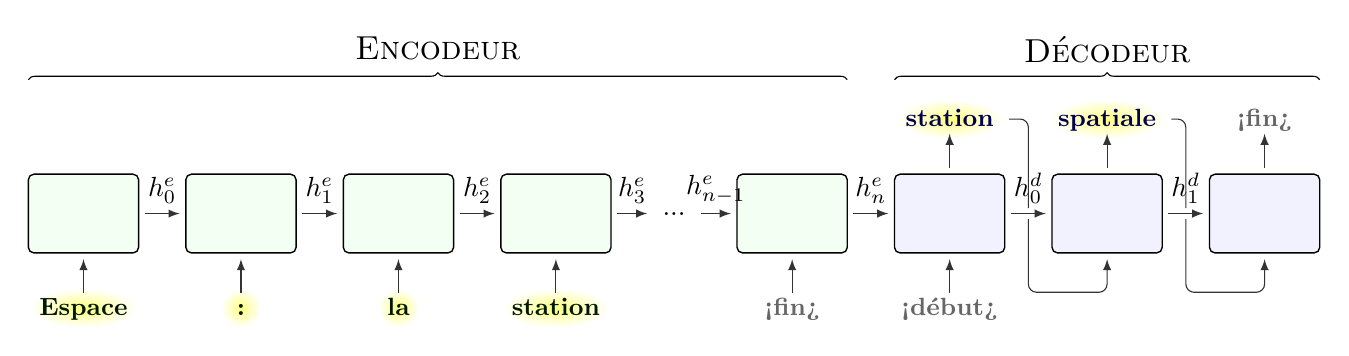
\begin{tikzpicture}

\tikzstyle{cell}=[text centered, rectangle, draw, line width=.5pt, minimum height=1cm, minimum width=1.4cm, rounded corners=2pt]
\tikzstyle{word}=[font=\small\bfseries, text centered, minimum size=.5cm, minimum height=.3cm, text height=1.5ex, text depth=.25ex]
\tikzstyle{vector}=[text centered, rectangle, draw, line width=.5pt, minimum height=.5cm, minimum width=1cm, rounded corners=2pt]
\tikzstyle{arrow}=[shorten >= 2pt, shorten <= 2pt, draw=black!80]

\node[cell, fill=enccolor] (E1) at (0,0){};
\node[cell, fill=enccolor] (E2) at (2,0){};
\node[cell, fill=enccolor] (E3) at (4,0){};
\node[cell, fill=enccolor] (E4) at (6,0){};
\node[text centered] (E5) at (7.5,0){...};
\node[cell, fill=enccolor] (E6) at (9,0){};

\node[word, color=inputcolor, inner color=yellow!50, outer color=white] (I1) at (0,-1.2){Espace};
\node[word, color=inputcolor, inner color=yellow!50, outer color=white] (I2) at (2,-1.2){:};
\node[word, color=inputcolor, inner color=yellow!50, outer color=white] (I3) at (4,-1.2){la};
\node[word, color=inputcolor, inner color=yellow!50, outer color=white] (I4) at (6,-1.2){station};
%\node[word, color=inputcolor, inner color=yellow!50, outer color=white] (I5) at (8,-1.2){...};
\node[word, color=startendcolor] (I6) at (9,-1.2){<fin>};

%\node[cell, fill=veccolor, word, rotate=90] (V) at (11,0){vecteur de pensée};

\node[cell, fill=deccolor] (D1) at (11,0){};
\node[cell, fill=deccolor] (D2) at (13,0){};
\node[cell, fill=deccolor] (D3) at (15,0){};
%\node[cell, fill=deccolor] (D4) at (20,0){};

\node[word, color=startendcolor] (I7) at (11,-1.2){<début>};
\node[word, color=outputcolor, inner color=yellow!50, outer color=white] (O1) at (11,1.2){station};
\node[word, color=outputcolor, inner color=yellow!50, outer color=white] (O2) at (13,1.2){spatiale};
\node[word, color=startendcolor] (O3) at (15,1.2){<fin>};

\draw[->,>=latex,arrow] (E1) -- (E2) node[above,midway] {$h^e_0$};
\draw[->,>=latex,arrow] (E2) -- (E3) node[above,midway] {$h^e_1$};
\draw[->,>=latex,arrow] (E3) -- (E4) node[above,midway] {$h^e_2$};
\draw[->,>=latex,arrow] (E4) -- (E5) node[above,midway] {$h^e_3$};
%\draw[->,>=latex,arrow] (E5) -- (E6) node[above,midway] {$h^e_{n-1}$};
\draw[->,>=latex,arrow] (E5) -- (E6) node[above,midway] {$h^e_{n-1}$};

\draw[->,>=latex,arrow,shorten <= -2pt] (I1) to (E1);
\draw[->,>=latex,arrow,shorten <= -2pt] (I2) to (E2);
\draw[->,>=latex,arrow,shorten <= -2pt] (I3) to (E3);
\draw[->,>=latex,arrow,shorten <= -2pt] (I4) to (E4);
%\draw[->,>=latex,arrow,shorten <= -2pt] (I5) to (E5);
\draw[->,>=latex,arrow,shorten <= -2pt] (I6) to (E6);
\draw[->,>=latex,arrow,shorten <= -2pt] (I7) to (D1);


\draw[->,>=latex, arrow] (E6) -- (D1) node[above,midway] {$h^e_n$};

\draw[->,>=latex,arrow] (D1) -- (D2) node[above,midway] {$h^d_0$};
\draw[->,>=latex,arrow] (D2) -- (D3) node[above,midway] {$h^d_1$};
%\draw[->,>=latex,arrow] (D3) to (D4);

\draw[->,>=latex,arrow,shorten >= -2pt] (D1) to (O1);
\draw[->,>=latex,arrow,shorten >= -2pt] (D2) to (O2);
\draw[->,>=latex,arrow,shorten >= -2pt] (D3) to (O3);
%\draw[->,>=latex,arrow,shorten >= -2pt] (D4) to (O4);

%\node at (5,2) {\large{\textsc{Encodeur}}};
%\node at (17,2) {\large{\textsc{Décodeur}}};

\draw[arrow, rounded corners=3pt] (O1) -| (12, 0);
\draw[->,>=latex, arrow, rounded corners=3pt] (12, 0) -- (12, -1) -| (D2.south);

\draw[arrow, rounded corners=3pt] (O2) -| (14, 0);
\draw[->,>=latex, arrow, rounded corners=3pt] (14, 0) -- (14, -1) -| (D3.south);

%\draw[arrow, rounded corners=3pt] (O3) -| (19, 0);
%\draw[->,>=latex, arrow, rounded corners=3pt] (19, 0) -- (19, -1) -| (D4.south);

\draw[decoration={brace},decorate] (-0.7,1.7) -- node[below=-1.9em] {\large{\textsc{Encodeur}}} (9.7,1.7);
\draw[decoration={brace},decorate] (10.3,1.7) -- node[below=-1.9em] {\large{\textsc{Décodeur}}} (15.7,1.7);


\end{tikzpicture}
}

\caption{Exemple de modèle \textit{encodeur-décodeur} récurrent appliqué à l'extraction automatique de mots-clés.}
\label{fig:seq2seq}
\end{figure}